\chapter{Calibration Of Low Cost Sensor}

With the development of sensor technology for air pollution it has attracted a majority of researchers as well as common people to explore and understand more about the pollutants and its effects. This has given freedom for one to set up their own monitoring system at residences, office or even at schools. The problem with this is to identify how accurate the data collected from these commodity sensors to the reference monitoring system. The reference system are the pollution monitoring devices that are developed to a clearly defined standard for a specific criteria pollutant [s] and has completed a rigorous testing and analysis protocol \cite{Hall2014}. If the system is giving values which is way too different from the reference value then it brings down the advantages of this technology. This issue can be dealt through calibration which will reduce the uncertainty in data and makes the output more accurate. 
\par 
Calibration can be defined as the act of evaluating and adjusting the precision and accuracy of measurement equipment \cite{Kejuruteraan2018}. If the measured output from the sensor is not equals to the actual output then it shows that there is a need for calibration. Usually all the electronic instruments are calibrated according to a particular conditions in the laboratory and acquires a certification of calibration before its sold out in the markets. Even then the measured value does not reach accuracy as the condition or the environment where it was calibrated changes that leaves the user with some raw values that gives no information. This issue was taken up and explored by a few researchers in the US Environmental Protection Agency(EPA) and suggested with three 'Straw-Man Approach' to improve the usability of such data and presented in the Air sensor Workshop \cite{Williams2013}. 

The first approach was by a signal-based calibration technique which requires the data from the remote stations, which is the reference station, to be broadcasted to the local station where the sensor is located and will receive this data and performs a single point calibration of the response. This approach would have been easy if the sensor was already equipped with the data collection and would process automatic calibration. 

The next option for calibrating is called the direct sensor calibration that involves placing the sensor in a chamber in which a known concentration of pollutant is set and response is observed. As the concentration of the pollutant is already known the output curve can be compared with it and calibrated accordingly. This is the most common method used for calibration as is often called as laboratory evaluation. Another way of approaching direct calibration is by inspecting the pre-defined response given by the manufacturer and checking how accurate the sensor is to the given concentration. In either case the calibration requires equipment and skills to give accurate concentration value.

The last option is by secondary data normalization in which the concentration values of the pollutant from the low cost sensor is normalized in accordance with the federal reference method (FRM) or federal equivalent method (FEM) analyzers. This approach is cost effective when compared to the other techniques and is less complex. This could be achieved by the use of a linear mathematical equation model that will convert the non-calibrated data into data of an acceptable form. The linear relationship equation $ y = mx + c $ where $ m $ is the slope and $ c $ is the intercept of the sensor raw data is compared with analyzer data and a relationship pattern is found out from this. The drawback of this is that the sensor data does not always give a linear response and thus not applicable for all the curves. 

Even though these 'Straw-Man Approach' was defined well it was still hard to implement it practically. This eventually led to the development of the 'Air Sensor Toolbox' by the Environmental Protection Agency (EPA) \cite{Williams2014} which introduced a tool called 'Macro Analysis Tool' (MAT) for performing comparisons of air sensor data with reference data and interpreting the results \cite{airsensorguidebook}.

\section{Calibration Procedure}

The Air Sensor Toolbox provide guidelines for researchers, citizen scientists and developers with working of low cost sensor and its calibration to give more insight about air quality \cite{airsensortoolbox}. The Air Sensor guidebook\cite{airsensorguidebook} provides a three step procedure for calibrating a sensor:
\begin{enumerate}
    \item Comparing the data from the low cost sensor with a reference instrument.
    
This means the data collected from the sensor system should be compared with the data from an already calibrated system which is placed by the local authority. This type of comparison is called as 'collocation' and in order to collocate, first find out where the reference system is placed and get access to the data from these system. After getting access to these system place the sensor system at the same level as the standard reference. Once this is done the data collected from both the system can be downloaded in the desired format.

    \item Creating a calibration curve with the help of Macro Analysis Tool (MAT).

The relationship between the response of an analytical instrument to the concentration or amount of an analyte introduced into a known instrument is referred to as the “calibration curve” \cite{Epa2010}. The MAT tool by EPA is used for drawing the calibration curve and will give an error function as output. This error function is an equation which can be used for calibrating the sensor.
    \item Repeating the calibration periodically.

    This procedure of calibration should be done periodically as the performance of instruments changes often. There will be changes in the equation and graph each time and this should be noted so as to get accurate value.
\end{enumerate} 

\section{Macro Analysis Tool -MAT}
The development of MAT tool gives a huge reliefs for the researchers in calibrating sensor data. This is an Excel based user-friendly macro tool that compares sensor data with reference data \cite{National2017} even if measurements weren’t recorded at precisely the same time, or were collected at different time intervals, such as 1-minute versus 5-minute intervals \cite{mattool}. The user needs to insert the data from the sensor into the sensor page of the tool and the values from the reference station is inserted into the reference page of the tool. After these values are inserted the details of pollutant, time interval, measurement units and data completeness (amount of usable data obtained) needs to be added in the set up page of the MAT. After all the required fields are filled the output page as shown in the figure \ref{MAT} shows the two sets of data being compared as per the control panel setting made in the tool \cite{National2017}.
This output page basically gives the statistical comparison of two different data sets. From this page it could be seen that the date and time stamps are averaged to a single value for both the system. There is another column in the sheet which is the invalid data points that gives the total number of non validated data points during the observed time. This non validated data points occurs due to either the fault by instrument or it could be the fault in reading by MAT or it could be even due to unacceptable range specified by the user.

\begin{figure}[h]
    \begin{center}
    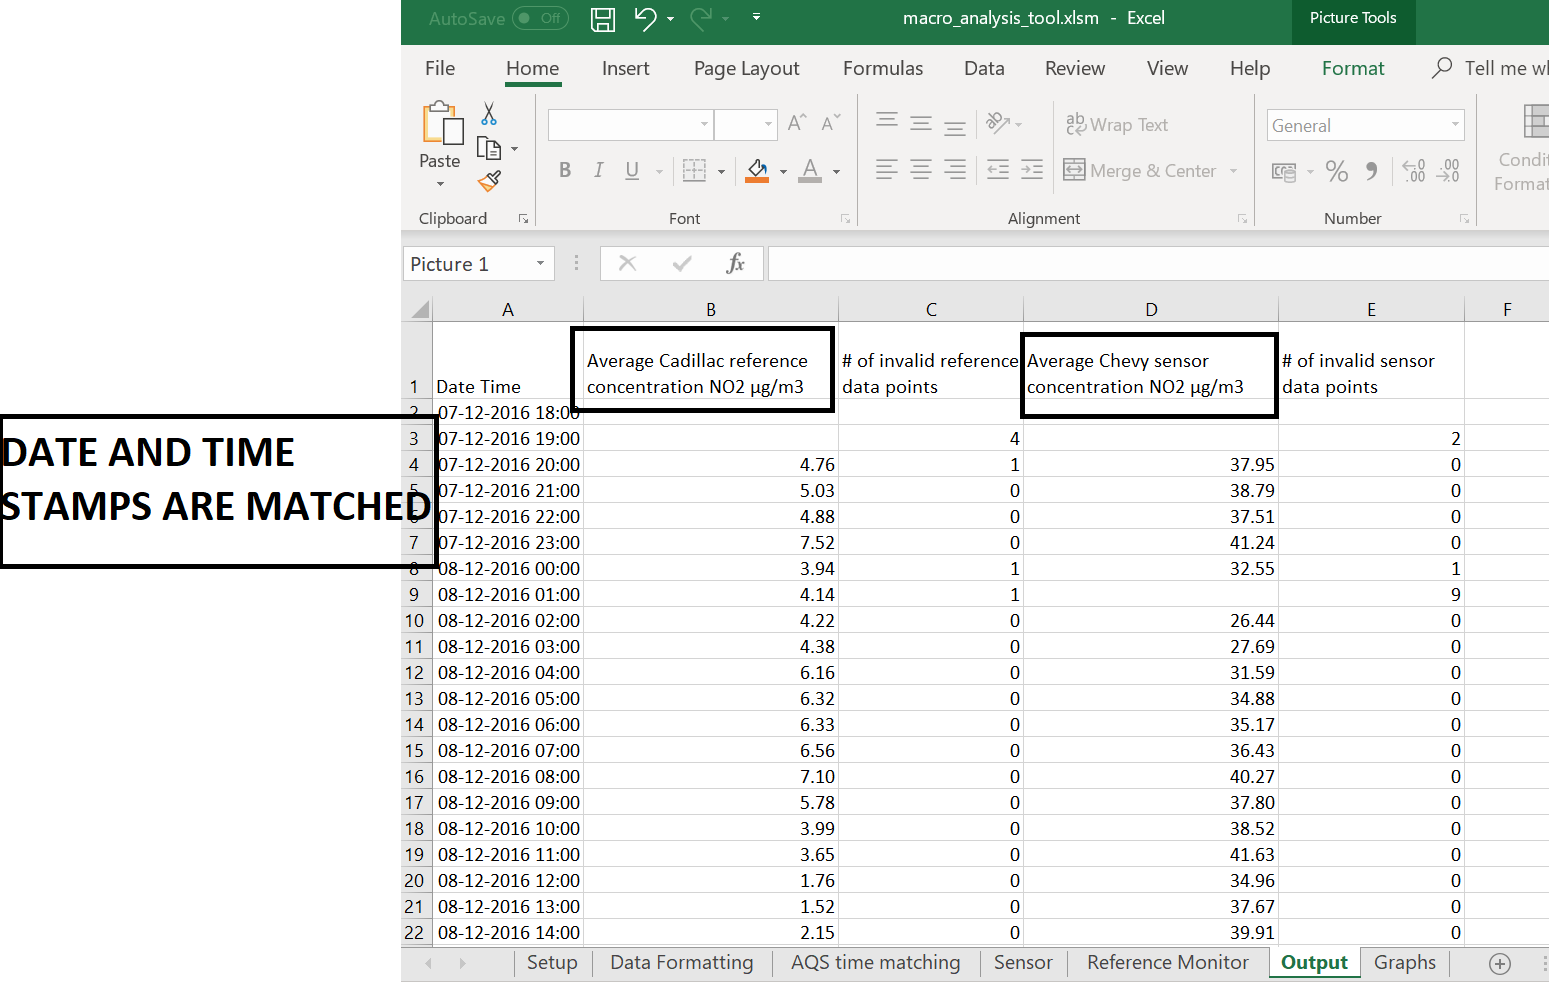
\includegraphics[scale=0.35]{./images/figure6.png}
    \end{center}
    \caption{MAT Output}
    \label{MAT}
  \end{figure}

 
\par
Another output page provided by the tool is correlation graph which plots a graph between the reference monitor and the sensor data as in the figure \ref{cor}.
The graph drawn will be a scatter plot and a line called as 'slope-intercept' will be drawn through the data points and is represented simply by the equation $ y = mx + c $. This equation represents the average behavior of the sensor data (vertical axis, represented by y) compared with the reference data (horizontal axis, represented by x) \cite{National2017}. The slope of the graph shows the similarity or difference in sensor measurements when compared with the reference instrument, on average. 

\begin{figure}[h]
    \begin{center}
    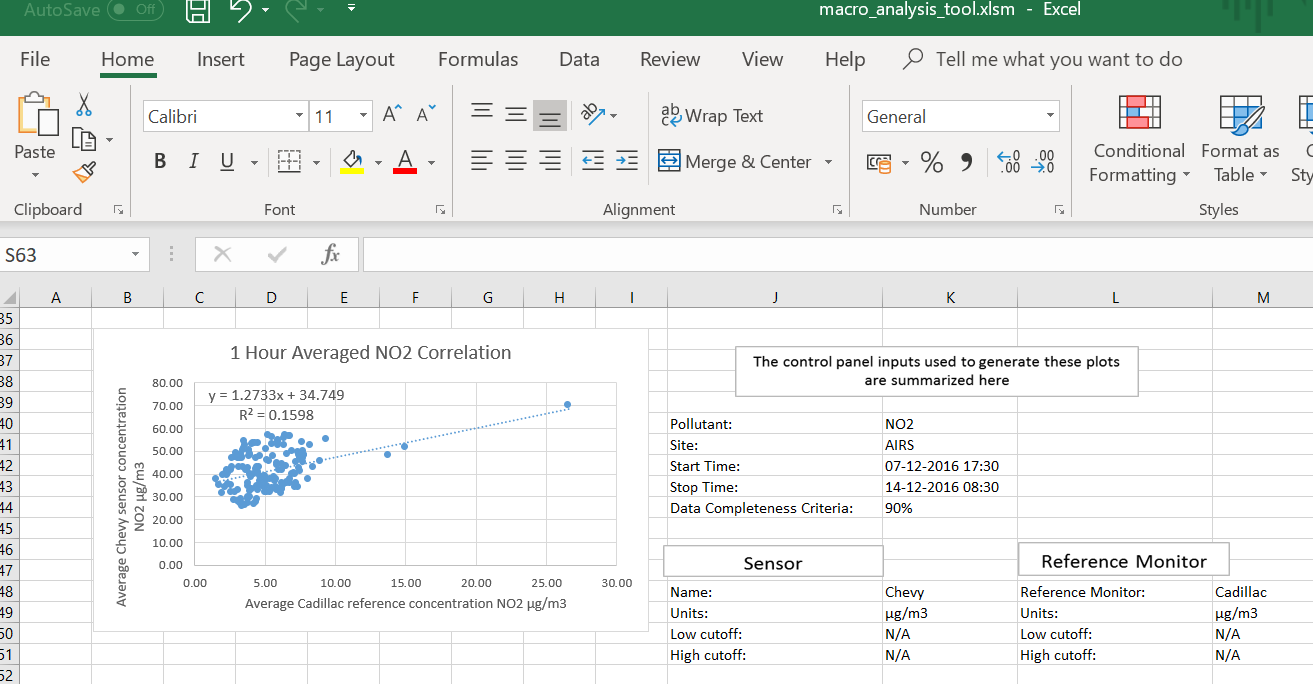
\includegraphics[scale=0.35]{./images/figure7.png}
    \end{center}
    \caption{Correlation Graph}
    \label{cor}
  \end{figure}

The tool also generates a coefficient of determination (also known as correlation coefficient in statistics) or R-Squared ($R^2 $) shows how close the value is to the slope-intercept line. The value ranges from 0 to 1 and the closer $R^2$ is to 1, the stronger the agreement between the sensor and the reference data \cite{Williams2018}. Along with these output the tool also generates a time series output graph which will show the concentration of pollutant for both the system as in the figure \ref{time}

\begin{figure}[h]
    \begin{center}
    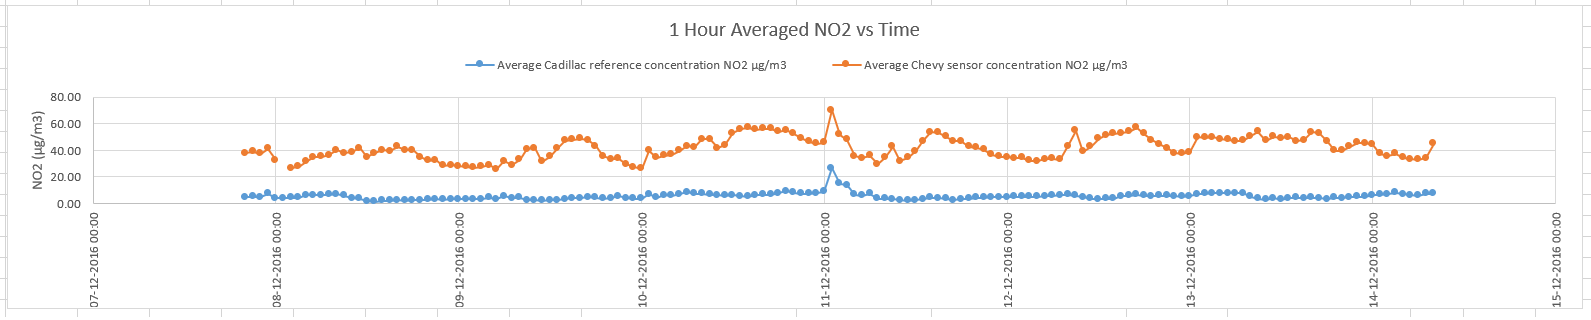
\includegraphics[scale=0.40]{./images/figure8.png}
    \end{center}
    \caption{Time-Series Graph}
    \label{time}
  \end{figure}

From the Time-Series graph it could be seen how the closely value from two different system is related to.
Having included all these functionality in the tool gives a strong solution for the calibration. The development of the tool was a year-long project of EPA with other community group(Clean Air
Carolina) and  one tribal nation(Eastern Band of Cherokee Indians). The next section will expand in detail about the background concept about the working of tool which is linear regression.

\section{Linear Regression}

Calibration can be done through different statistical methods and the most popular approach is Linear Regression method. In statistics, the term regression is used to describe a group of methods that summarize the degree of association between one variable (or set of variables) and another variable (or set of variables) \cite{Burke}. Linear Regression establishes relationship between two variables one is the independent variable which will be on the $x$ axis and the dependent variable in the $y$ axis by drawing a straight line.
If there are many observations and is plotted as a scatter plot then a line called as regression line as in the figure \ref{LRM} could be drawn through it by Least Square method. 


\begin{figure}[h]
    \begin{center}
    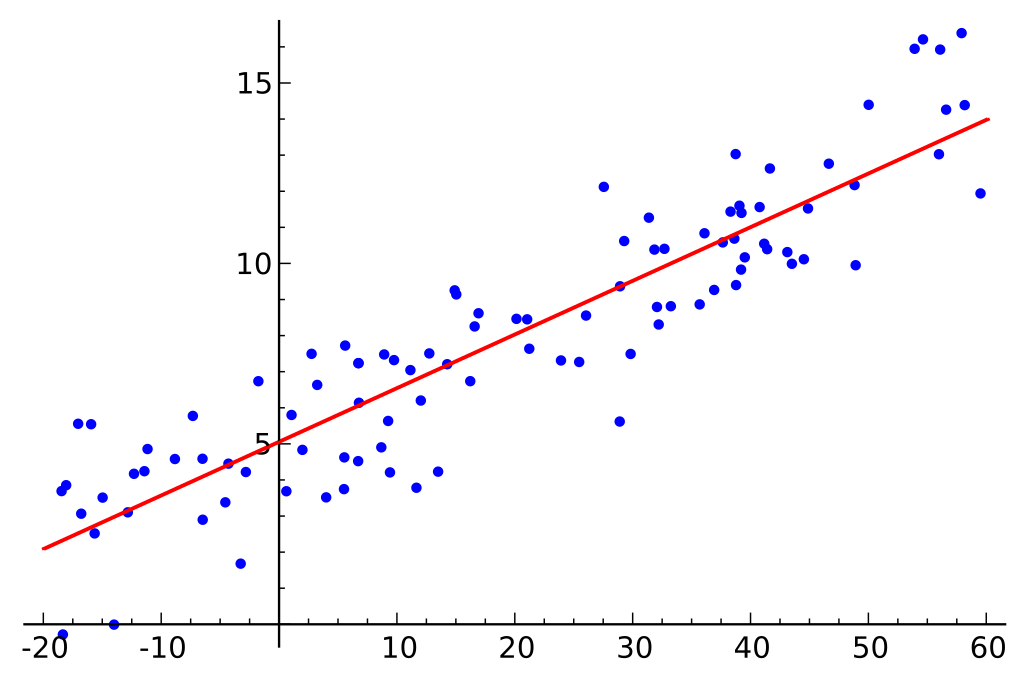
\includegraphics[scale=0.25]{./images/figure9.png} 
    \end{center}
    \caption{Linear Regression Model \cite{regression}}
    \label{LRM}
  \end{figure}
  The method of Least Squares is a procedure to determine the best fit line to data\cite{S.Miller1992} by minimizing the errors between the observed value and the actual value. This method considers that, for each value of $x$, there is a sub-population of $y$ values normally distributed, that the means of all the sub-populations of $y$ lie on the same straight line and all the sub-populations of $y$ values have equal variances \cite{Almeida2002} \cite{daniel2018biostatistics}.
  The line drawn will have a slope $m$ and is given by the formula
\begin{center}

    
             {\large  $ m = \frac{\sum_{i}[(x_i-\bar{x})(y_i-\bar{y})]}{[ \sum_{i}(x_i-\bar{x})^2 ]}$} \cite{Stone2001} \cite{Arsova2009} \cite{Burke}


\end{center}
where $m$ is the slope, $x_i$ and $y_i$ are the reference and observed data values, $\bar{x}$ and $\bar{y}$ are the mean values of the data. The mean values will act as the centroid of the regression line and it has to pass through these points.
The intercept equation $c$ is

\begin{center}
 
    { $ C = \bar{y}-m\bar{x}$} \cite{Stone2001} \cite{Harvey2016}

\end{center}

On getting the slope and intercept value the equation of line can be found. Once the Regression line is drawn, to find out how much the data is scattered and to what extend, correlation coefficient ($R^2$) is used. In other words $R^2$ gives the measure of  degree to which the values of x and y are linearly correlated \cite{Stone2001}. The equation for finding the regression value is

\begin{center}

    {\large $R^2 = \frac{\sum_i[(x_i-\bar x)(y_i-\bar y)]}{\sqrt{[\sum_i(x_i-\bar x)^2[\sum_i(y_i-\bar y)^2]]}}$ } \cite{Stone2001}

\end{center}
The range of value for $R^2$ is between 0 to 1 and closer the value is to 1, the stronger the correlation between the two data.
All these equation can be easily calculated with the help of Excel and thus all these equations are integrated to the MAT tool.


